\section{Position and Orientation}
\subsection{Introduction}
Kinematics studies the movement of an object -- in our case of a robot -- without taking into acount the forces generating it. Instead, it only handles aspects such as position, orientation, speed and momentum of bodies in movement.

Consider for instance a robotic arm. We can design a simplified scheme of the robot and its environment, to create a kinematic pipeline and reference frames associated to each of these objects.

\begin{figure}[H]
    \centering
    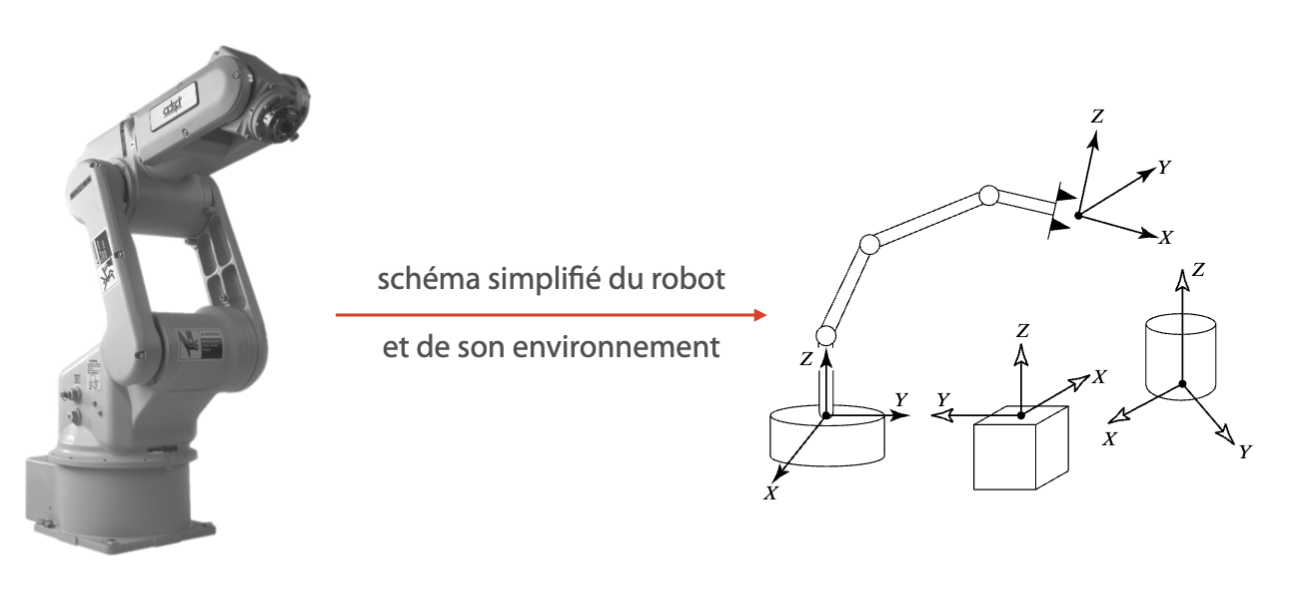
\includegraphics[width=.6\textwidth]{position/arm-scheme.png}
    \caption{Simplified scheme of the robot feature the kinematic pipeline and reference frames.}
\end{figure}

\emph{Direct kinematics} allows to compute the position and orientation of the terminal organ given, for instance, the angles of the articulations.

\begin{figure}[H]
    \centering
    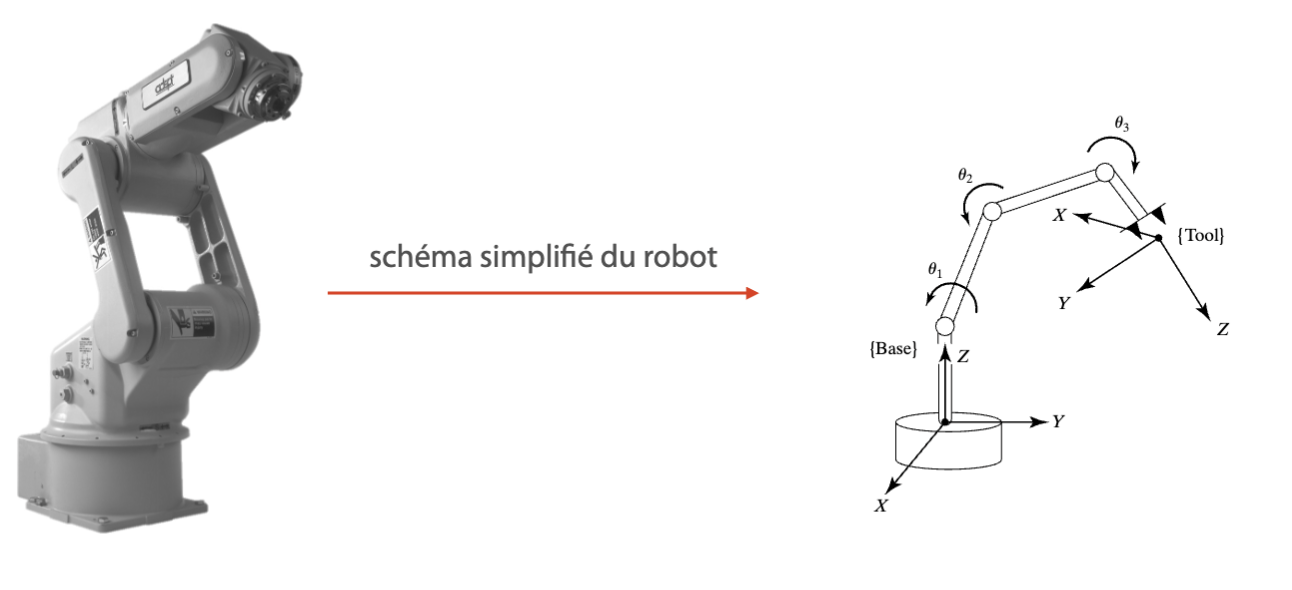
\includegraphics[width=.6\textwidth]{position/direct-kinematic.png}
\end{figure}

\emph{Invert kinematics} answers the question the other way around: given the position and orientation of a boyd, how can we compute the values of the articulations angles. Invert kinematics is used for instance for trajectory tracking: given a reference trajectory, how can we compute the speed of the articulations?

\subsection{Position of a point in space}
Once that a frame of reference $\{A\}$ is defined, we can localize any point of the universe given a \emph{position vector}:
\begin{figure}[H]
    \centering

    \begin{minipage}{0.4\textwidth}
        \begin{equation*}
            \prescript{A}{}{P} = \begin{bmatrix}
                p_x \\ p_y \\ p_z
            \end{bmatrix}
        \end{equation*}
    \end{minipage}
    \begin{minipage}{0.4\textwidth}
        \centering
        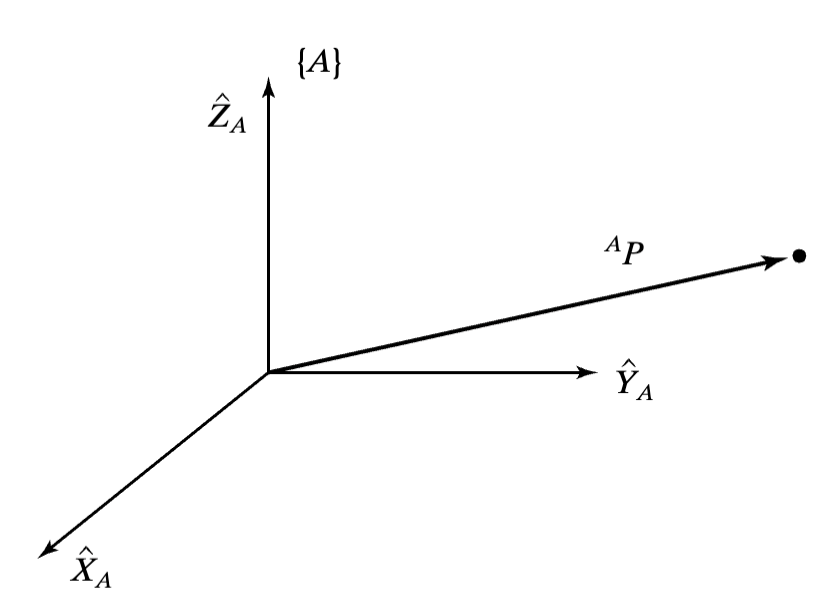
\includegraphics[width=.8\textwidth]{position/position-frame.png}
    \end{minipage}
    \caption{Vector and position of the point established in the frame $\{A\}$.}
\end{figure}